\documentclass{article}
\usepackage{tikz, comment}
\usepackage{pifont}
\usepackage{fontspec}
\usetikzlibrary{arrows, decorations.markings, decorations.pathreplacing}
\begin{comment}
:Title: Not defined yet
:Tags: area using polar coordinates, polar integral formula ;polar form of a complex number;cardioid;polar coordinates;cis
:Prob: 0.583;0.4523;0.4041;0.3987;0.3624
:Author: Prof.Hu Ji-shan, HKUST
:Slug: No name yet

Description Here.........
\end{comment}
\begin{document}\centering

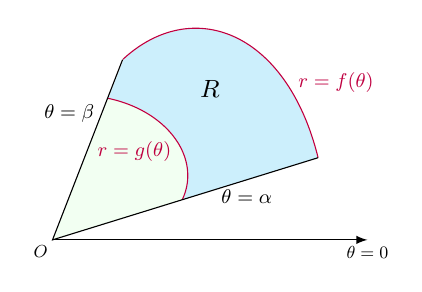
\begin{tikzpicture}[>=latex,xscale=.5*0.8, yscale=.5*0.8][font=\sf\small]

\draw[->] (0, 0) -- (10, 0)node[below, scale=0.7] {$\theta=0$};

\node[scale=0.7] at (-0.3/0.8, -0.3/0.8) {$O$};

\draw[white, fill=cyan!20, samples=100, smooth, domain= 0.3:1.2, variable=\t]
plot ({8*((cos(\t r)-1.2)^3-0.4*(cos(\t r))+1.5)*cos(\t r)}, {8*((cos(\t r)-1.2)^3-0.4*(cos(\t r))+1.5)*sin(\t r)})--(0,0) ;

\draw[purple, samples=100, smooth, domain= 0.3:1.2, variable=\t]
plot ({8*((cos(\t r)-1.2)^3-0.4*(cos(\t r))+1.5)*cos(\t r)}, {8*((cos(\t r)-1.2)^3-0.4*(cos(\t r))+1.5)*sin(\t r)});

\draw[white, fill=green!5!white, samples=100, smooth, domain= 0.3:1.2, variable=\t]
plot ({3*((sin(\t r)-1.0)^3+0.3*(cos(\t r))+1.5)*cos(\t r)}, {3*((sin(\t r)-1.0)^3+0.3*(cos(\t r))+1.5)*sin(\t r)})--(0,0) ;

\draw[purple, samples=100, smooth, domain= 0.3:1.2, variable=\t]
plot ({3*((sin(\t r)-1.0)^3+0.3*(cos(\t r))+1.5)*cos(\t r)}, {3*((sin(\t r)-1.0)^3+0.3*(cos(\t r))+1.5)*sin(\t r)});

\draw ({8*((cos(0.3 r)-1.2)^3-0.4*(cos(0.3 r))+1.5)*cos(0.3 r)}, {8*((cos(0.3 r)-1.2)^3-0.4*(cos(0.3 r))+1.5)*sin(0.3 r)}) -- (0, 0) node[below, xshift=3, pos=0.3, scale=0.8]{$\theta=\alpha$}
--
({8*((cos(1.2 r)-1.2)^3-0.4*(cos(1.2 r))+1.5)*cos(1.2 r)}, {8*((cos(1.2 r)-1.2)^3-0.4*(cos(1.2 r))+1.5)*sin(1.2 r)}) node[left, pos=0.7, scale=0.8] {$\theta=\beta$};

\node[purple, scale=0.8] at (9, 5) {$r = f(\theta)$};
\node[purple, scale=0.8] at (2.6, 2.8) {$r = g(\theta)$};

\node[scale=1] at (5, 4.8) {$\mathscr R$};

\end{tikzpicture}
\end{document}